\documentclass[
  11pt,
  letterpaper,
   addpoints,
   answers
  ]{exam}

\usepackage{../exercise-preamble}
\usepackage{float}

\begin{document}

\noindent
\begin{minipage}{0.47\textwidth}

\includegraphics[width=\textwidth]{../fcfm_die}
\end{minipage}
\begin{minipage}{0.53\textwidth}
\begin{center} 
\large\textbf{Fundamentos de control de sistemas} (EL4111-1) \\
\large\textbf{Pauta control 2} \\
\small Prof.~Roberto Cardenas Dobson\\
\small Prof.~Aux.~Osvaldo Jimenez - Erik Sáez\\
\small Ayudantes.~Simon Arenas- Juan Pablo Baez - Francisco Garces - Sofia Ibarra\\
\end{center}
\end{minipage}

\vspace{0.5cm}
\noindent
\vspace{.85cm}

\begin{questions}
   %-------------------------
    \question Se tiene el siguiente sistema de control digital:
    \begin{figure}[h!]
        \centering
        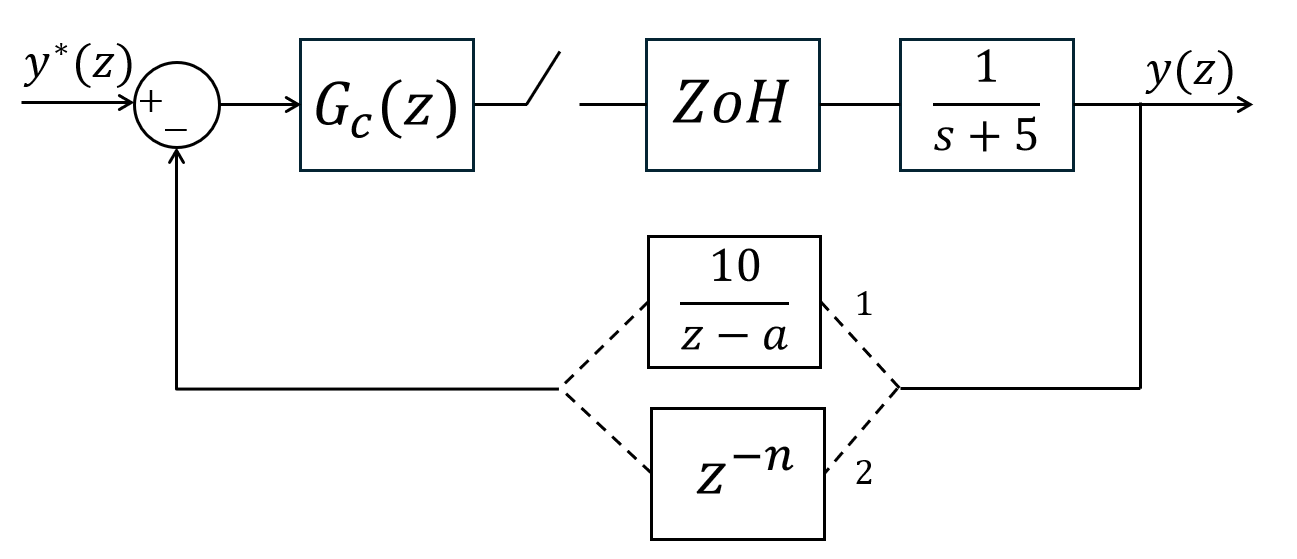
\includegraphics[width=0.6\linewidth]{Control_2_1}
    \end{figure}
    En el lazo de retroalimentación se tiene un sistema inalámbrico de transmisión de datos que, dependiendo de las condiciones atmosféricas, puede introducir un retardo de $n$ muestras en el sistema de control (estado 2). Para efectos de diseño, se desea que la respuesta del sistema de control a diseñar cumpla con los requerimientos de coeficiente de amortiguamiento $\xi=0.8$ y de una frecuencia natural de $\omega_n=60 [rad/s]$. La frecuencia de muestreo es de $\omega_s=15\omega_n$. Utilizando la transformada exacta de $Z$, se le pide resolver las siguientes preguntas.
    \begin{enumerate}
    \item Implemente un controlador proporcional de la forma $G(z)=K$. Considere que, operando en el estado 1, existe la posibilidad de cambiar el valor del polo del lazo de retroalimentación del sistema de transmisión de datos ¿Qué condición debe cumplir $a$ para que el sistema pueda alcanzar los requerimientos de diseño con este controlador? Utilice LGR para encontrar el valor de $a$ y de $K$. (15/100)
    \item ¿Existe la posibilidad de que el sistema se haga inestable para algún valor de $K$? De ser así, encuentre el valor de $K$ del controlador de a) que produce inestabilidad. (15/100)
    \item Considere ahora que el sistema inálamabrico de transmisión de datos está operando en el estado 2, con $n=1$. Diseñe un controlador que permita cumplir las especificaciones originales y alcanzar cero error en estado estacionario a entrada escalón (15/100).
    \end{enumerate}
%----------------------------------
\begin{solution}
    \subsection*{Resolucion (1.1)}
    Dado que inicialmente se esta operando en el estado 1, lo primero a realizar sera aplicar la transformada Z exacta al sistema, considerando el ZoH
    \begin{align}
        Z_{planta}(z) &= Z\left\{\frac{1-e^{sT}}{s} \cdot \frac{1}{s+5}\right\} \\
        &= \frac{z-1}{z} \cdot Z\left\{\frac{1}{s} \cdot \frac{1}{s+5}\right\}\\
        &= \frac{z-1}{5z} \cdot Z\left\{ \frac{1}{s} - \frac{1}{s+5}\right\}\\
        &= \frac{z-1}{5z} \cdot \left( \frac{z}{z-1} - \frac{z}{z-e^{-5T}}\right)\\
        &= \frac{0.00685}{z-0.9657}
    \end{align}    
    Esto considerando que el tiempo de muestreo viene dado por:
    \begin{align}
        T_{s} = \frac{2\pi}{15\cdot w_{n}} = 0.00698
    \end{align}
    Con esto tenemos que la funcion a lazo abierto corresponde a tanto el lazo de retroalimentación como a la planta discretizada, es decir:
    \begin{align}
        G(z) \cdot H(z) = K \cdot \frac{0.0685}{(z-0.9657)(z-a)}
    \end{align}
    Teniendo los valores de ambos polos y conociendo el valores de $\xi$ y $\omega_{n}$, se tiene que que el punto de diseño en Z sera:
    \begin{align}
        Z_{1,2}^{*} &= e^{T_{s}(- 0.8 \cdot 60 \pm j60 \sqrt{1-(0.8)^{2}})}\\
        &= 0.6929 \pm j0.1778
    \end{align}
    Con lo que el LGR vendra dado por lo siguiente:
    \begin{center}
        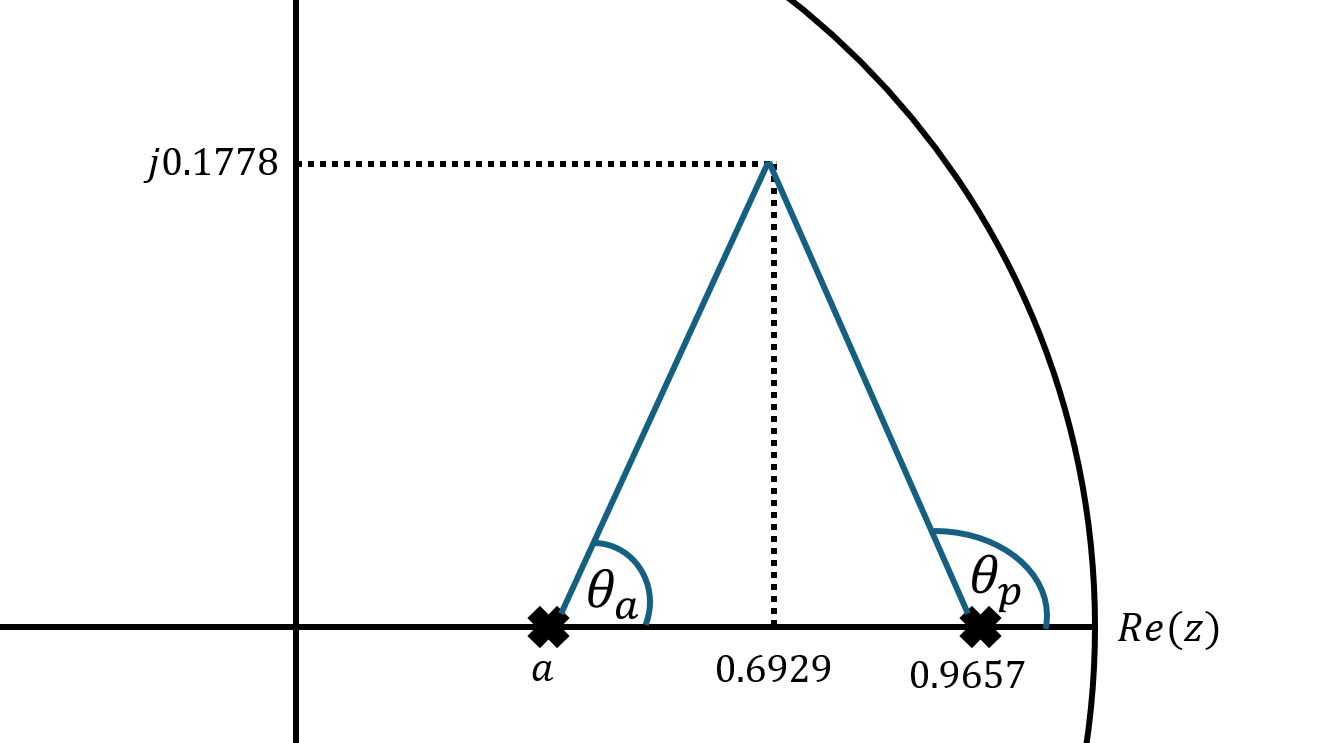
\includegraphics[width=0.4\textwidth]{Control_2_2.png}
        \captionof{figure}{LGR del sistema de lazo cerrado}
    \end{center}
    Se tendra por tanto que:
    \begin{align}
        \theta_{p} &= 180^{\circ} - tan^{-1}\left( \frac{0.1778}{0.9657-0.6929}\right)=146.91^{\circ}\\
        \theta_{a} &= tan^{-1}\left(\frac{0.1778}{0.6929-a}\right)
    \end{align}
    Por condicion de angulo tenemos que:
    \begin{align}
        \theta_{a} = 180^{\circ} - \theta_{p} = 33.09^{\circ}
    \end{align}
    Se obtiene por tanto el valor de a como:
    \begin{align}
        tan(33.09^{\circ}) &= \frac{0.1778}{0.6929-a}\\
        a &= 0.42005 
    \end{align}
    Lo anterior puede verificarse debido a la forma conocida del LGR, en la que se debera cumplior que la distancia de \textbf{a} a la parte real del punto de diseño sea igual a la distancia de la parte real del polo a la parte real del punto de diseño.Luego calculamos la ganancia que es necesaria, obteniendose lo siguiente:
    \begin{align}
        K &= \left| \frac{1}{\frac{0.0685}{(z-0.9657)(z-0.42)}}\right|_{z=z*}\\
          &=1.5483
    \end{align}
    \subsection*{Resolucion (1.2)}
    Se busca analizar la inestabilidad del sistema, dada la forma del LGR, tendremos que este divergera unicamente en la vertical, por lo tanto se tendra que el sistema sera criticamente estable cuando se intersecte la circunferencia unitaria, se visualiza de la siguiente manera:
    \begin{center}
        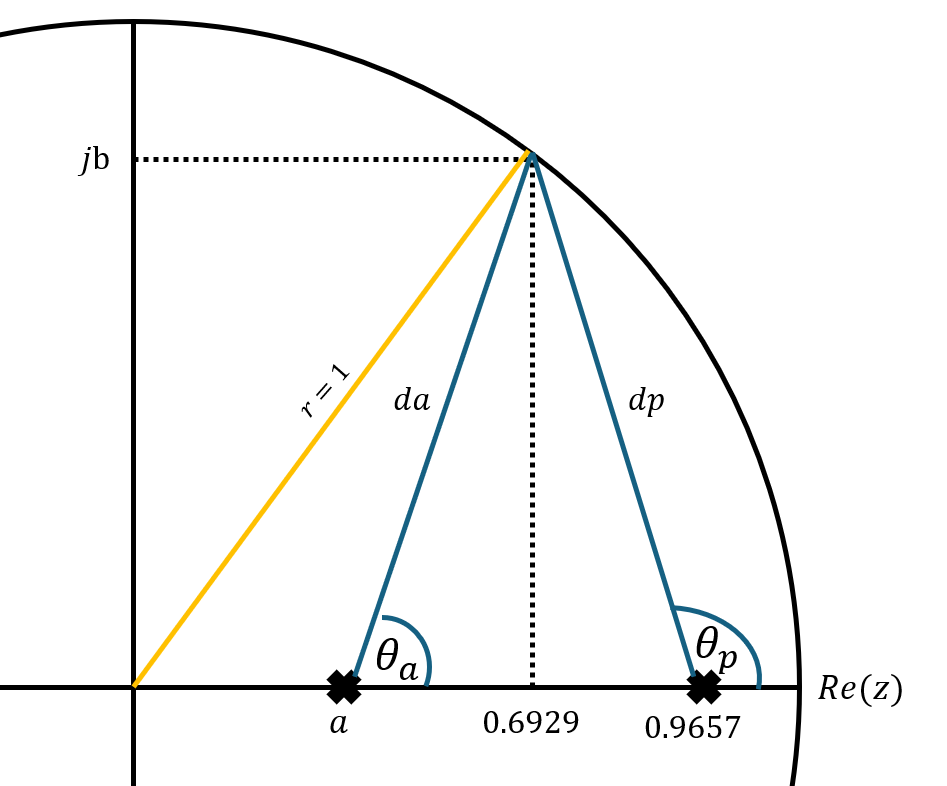
\includegraphics[width=0.5\textwidth]{Control_2_3.png}
        \captionof{figure}{LGR del sistema de lazo cerrado}
    \end{center}
    Se tendra que la distancia horizontal \textbf{b} a la que sera criticamente estable corresponde a:
    \begin{align}
        b= \sqrt{1- 0.6929^{2}} = 0.721
    \end{align}
    Con lo que la ganancia del sistema vendra dada por lo siguiente:
    \begin{align}
        K_{sys} = \frac{\prod \text{Distancia polos}}{\prod \text{Distancia ceros}}
    \end{align}
    De esta manera dado que no existen ceros, este valdra 1. Por tanto tenemos que:
    \begin{align}
        K_{sys} &= \frac{da \cdot dp}{1}\\
        &= \frac{\sqrt{0.42^{2} + 0.72103^{2}} \cdot \sqrt{0.42^{2} + 0.72103^{2}}}{1}\\
        &= 0.6963
    \end{align}
    Pero tenemos que tener en cuenta que este es el $k_{sys}$ es del sistema por lo que:
    \begin{align}
        K_{sys} &= 0.6963 \\
                &= K \cdot 0.0685\\
        K &= 10.1649
    \end{align}
    De esta manera se obtiene el valor de k critico para el cual el sistema es inestable
    \subsection*{Resolucion (1.3)}
    Dado que el sistema ahora opera en el estado 2 y ademas tiene un retardo de 1 muestra (n = 1), luego tendremo que el controlador propuesto sera tal que:
    \begin{align}
        G_{c}(z) = K \cdot \frac{(z-a)}{z-1}
    \end{align} 
    Con lo que se tiene que el sistema a lazo abierto vendra dado por:
    \begin{align}
        G(z) \cdot H(z) = K \cdot \frac{(z - a)}{z - 1} \cdot \frac{0.0685}{(z-0.9657)} \cdot \frac{1}{z}
    \end{align}
    Con lo que tenemos que el LGR vendra dado por:
    \begin{center}
        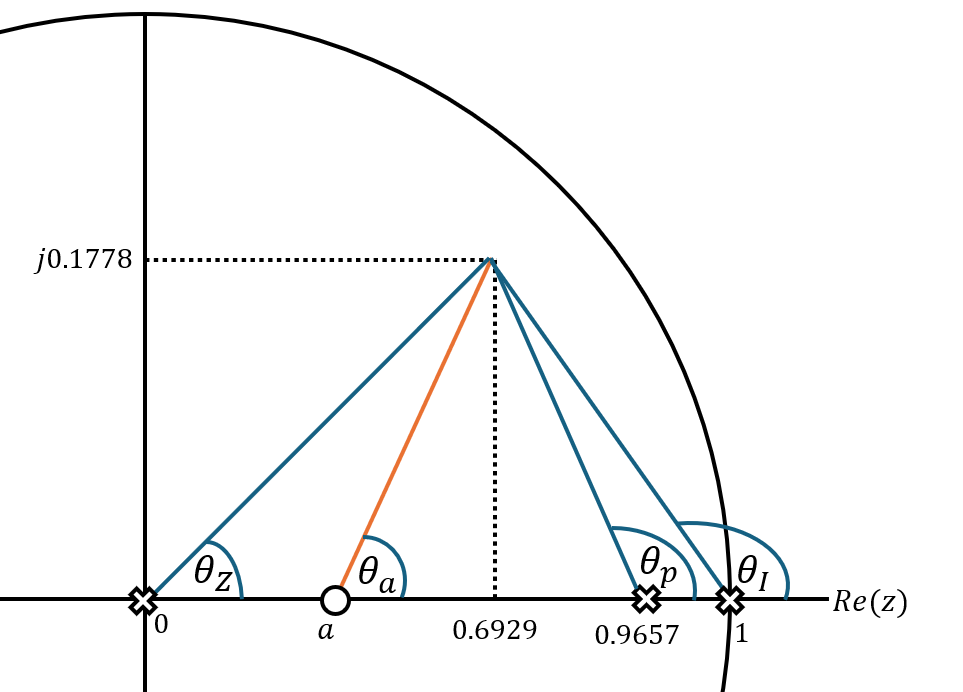
\includegraphics[width=0.5\textwidth]{Control_2_4.png}
        \captionof{figure}{LGR del sistema de lazo cerrado}
    \end{center}
    De esta manera se tendra que por condicion de angulo:
    \begin{align}
        \theta_{I} + \theta_{P} + \theta_{z} - \theta_{a} = 180^{\circ}
    \end{align}
    Donde se tiene que:
    \begin{align}
        \theta_{I} &= 180^{\circ} - tan^{-1}\left(\frac{0.1778}{1- 0.6929}\right) = 149.93^{\circ}\\
        \theta_{P} &= 180^{\circ} - tan^{-1}\left(\frac{0.1778}{0.9657-0.6929}\right) = 146.91^{\circ}\\
        \theta_{z} &= tan^{-1}\left(\frac{0.1778}{0.6929}\right) = 14.39^{\circ}\\
        \theta_{a} &= tan^{-1}\left(\frac{0.1778}{0.6929-a}\right)
    \end{align}
    De esta manera se obtiene que:
    \begin{align}
        \theta_{a} & = \theta_{I} + \theta_{P} + \theta_{z} - 180^{\circ} = 131.23^{\circ}
    \end{align}
    Con lo que finalmente:
    \begin{align}
        tan(\theta_{a}) &= \frac{0.1778}{0.6929-a}\\
        a &= 0.53708 
    \end{align}
    Con lo que la ganancia sera:
    \begin{align}
        K = \left| \frac{1}{\frac{(z-0.53708)\cdot 0.0685 }{(z-1)(z-0.9657)z}}\right|_{z=z^{*}} = 5.10413
    \end{align}
    De esta manera se tendra que el controlador sera de la forma:
    \begin{align}
        G_{c}(z) = 5.10413 \cdot \frac{(z-0.53708)}{z-1}
    \end{align}
\end{solution}
\newpage
%----------------------------------
    \question 
    Se tiene la siguiente planta, que se utiliza con un control proporcional y una frecuencia de muestreo de $1\,$kHz:
    
    \begin{equation}
        G_p(z) = \frac{1}{(z-0.5)^3} \tag{1}
    \end{equation}
    
    Se pide:
    
    \begin{enumerate}
        \item[i)] Dibuje el lugar de la raíz y encuentre la frecuencia natural de los polos complejos de lazo cerrado, en el plano $z$, cuando operan con un coeficiente de amortiguamiento igual a cero. (12/100)
        
        \item[ii)] Si se obtiene un polo real en el plano $z$. ¿Es posible operar con un coeficiente de amortiguamiento de $\zeta = 0.707$ con este polo? (12/100) Si fuera posible, ¿Qué valor de ganancia se necesitaría?
    \end{enumerate}
    
    (b) Se desea controlar las plantas cuyas respuestas en frecuencia se encuentran en la tabla. El sistema a controlar se encuentra en la figura y está compuesto de dos plantas de primer orden. La realimentación utiliza un canal de comunicaciones que opera con una frecuencia de muestreo de $100\,$Hz. Se pide:
    
    \begin{enumerate}
        \item[i)] Suponiendo que el sistema funciona con $n=0$, diseñe un controlador proporcional que entregue un coeficiente de amortiguamiento de $\zeta = 0.56$. (14/100)
        
        \item[ii)] Se congestiona el sistema y existe un retardo de una muestra. Diseñe una red en adelanto que mantenga operación con el mismo margen de fase y frecuencia de cruce lograda en i). Utilice cancelación aproximada del polo más lento o el método de inyección de máxima fase. (17/100)
    \end{enumerate}
    \begin{figure}[h!]
        \centering
        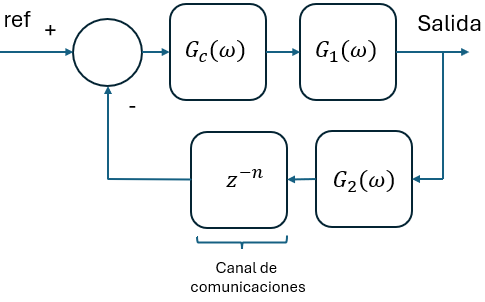
\includegraphics[width=0.4\textwidth]{Control_2_5.png}
        \caption{Esquema del sistema de control}
    \end{figure}
    
    \begin{table}[H]
        \centering
        \caption{Datos de magnitudes y fases.}
        \begin{tabular}{c|c|c|c|c}
            $\omega$ & Mag 1 & Fase 1 & Mag 2 & Fase 2 \\ \hline
            0 & 0.333333333333 & -18.434948822922006 & 0.0666666666667 & -3.814074834290351 \\
            1 & 0.316227766017 & -33.690067525979785 & 0.066519010523737 & -7.594643368591441 \\
            2 & 0.277350098112615 & -45.00000000000000 & 0.066081860450095 & -11.309932474020208 \\
            3 & 0.235702260395516 & -53.130102354155980 & 0.065374202054660 & -14.931417178137542 \\
            4 & 0.200000000000000 & -59.036243467926482 & 0.064415562620038 & -18.434948822922006 \\
            5 & 0.171498585142509 & -63.434948822922010 & 0.063245553203368 & -21.801409486351812 \\
            6 & 0.149071198499986 & -66.801409486351815 & 0.061898445060017 & -25.016893478100013 \\
            7 & 0.131306432859723 & -69.443954780416533 & 0.060412203933415 & -28.072486935852954 \\
            8 & 0.117041147196131 & -71.565051177077990 & 0.058822941177655 & -30.963756532073521 \\
            9 & 0.105409255338946 & -73.300755766006375 & 0.057166619504750 & -33.690067525979785 \\
            10 & 0.095782625221145 & -74.744881296942225 & 0.055470192622523 & -36.253837377447909 \\
            11 & 0.087705819307033 & -75.963756532073518 & 0.053760353570477 & -38.659082540090088 \\
            12 & 0.080845208345444 & -77.053083262683995 & 0.052057920629535 & -40.914383220555130 \\
            13 & 0.074953168899865 & -77.905242292878795 & 0.050358332083818 & -43.025000518901919 \\
            14 & 0.069843029576062 & -78.690067525979785 & 0.048733444072887 & -45.000000000000000 \\
            15 & 0.065372045046060 & -79.380347238848711 & 0.047140452079013 & -46.847610265994598 \\
            16 & 0.061429511683493 & -79.992020195858469 & 0.045609675258575 & -48.576334749979994 \\
            17 & 0.057928446364347 & -80.537977919747347 & 0.044151037324348 & -50.193554897427874 \\
            18 & 0.054797652433260 & -81.027733381031601 & 0.042769033331288 & -51.709836773656673 \\
            19 & 0.051987521345219 & -81.469234390051867 & 0.041467890712558 & -53.130102354155980 \\
            20 & 0.049446817643415 & -81.863757493186823 & 0.040250472901170 & -54.458121105185058 \\
        \end{tabular}
        \label{tab:datos}
    \end{table}
    
        
%------------------------
\begin{solution}
\subsection*{Resolucion (a-i)}
Dada que se busca dibujar el LGR y encontrar la frecuencia natural de los polos complejos, se tiene que la funcion a lazo abierto vendra dada por:
\begin{center}
    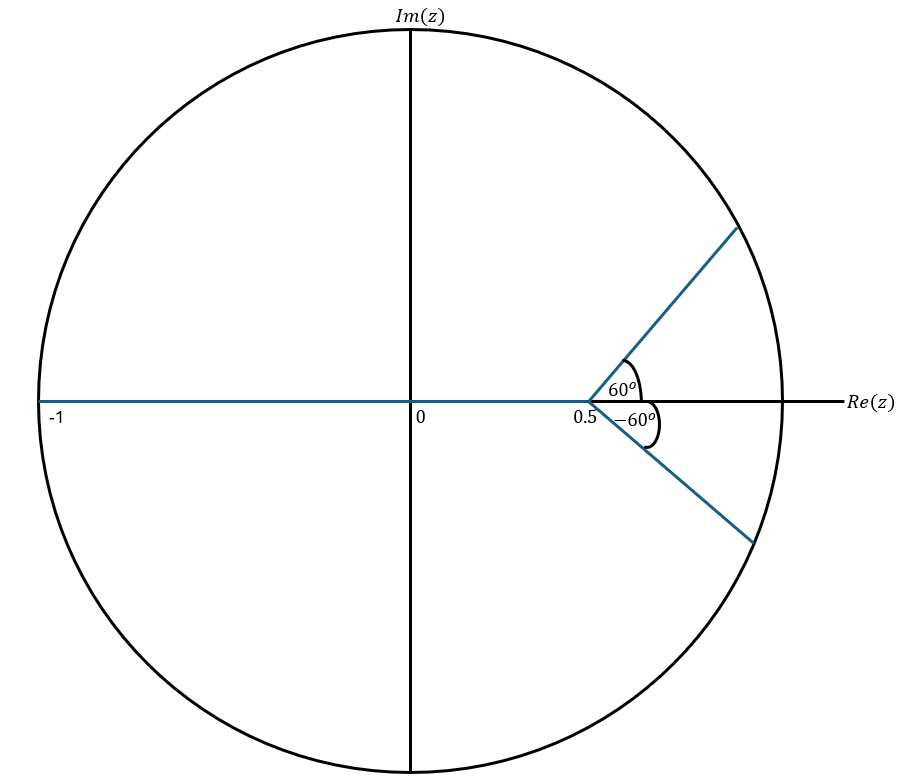
\includegraphics[width=0.5\textwidth]{Control_2_6.png}
    \captionof{figure}{LGR del sistema de lazo cerrado}
\end{center}
Donde es posible obtener algunas caracteristicas del LGR dadas por:
\begin{align}
    \text{N Asintotas} = N_{p} - N_{z} = 3 - 0 = 3
\end{align}
Luego para el angulo tenemos que:
\begin{align}
    \angle \theta_{a} = \frac{(2k+1)\pi}{N_{p}-N_{z}} = \frac{(2k+1)\pi}{3}
\end{align}
Dando el rango de asintotas por $\theta_{a} \in \left\{ \frac{\pi}{3}, \pi , \frac{5\pi}{3}\right\}$. Luego se debe tener en consideracion que:
\begin{align}
    s= \frac{1}{T} (ln(r) + \pm j\theta)
\end{align}
Dado que se nos menciona por enunciado que el coeficiente de amortiguamiento es nulo, se tendra que:
\begin{align}
    s^{*}_{1,2} = -\xi w_{n} \pm jw_{n} = \pm jw_{n}
\end{align}
Con lo que el punto de diseño vendra dado por:
\begin{align}
    z_{1,2}^{*} = e^{T_{s}(jw_{n})}
\end{align}
Un resultado muy importante de lo anterior, esque se tendra que los polos se ubicaran \textbf{en la circunferencia unitaria}, considerando que (Z=-1) que es es la ubicacion de unos de los polos, que escrito como $Z_{1,2}^{*} = re^{\theta}$ tendremos que $\theta = \pi$ con lo que se logra obtener la relacion dada por:
\begin{align}
    T_{s}\omega_{n} &= \pi\\
    \omega_{n} &= \frac{\pi}{T_{s}} = 3141.59[rad/s]
\end{align}
Para los otros polos se tendra el siguiente esquema:
\begin{center}
    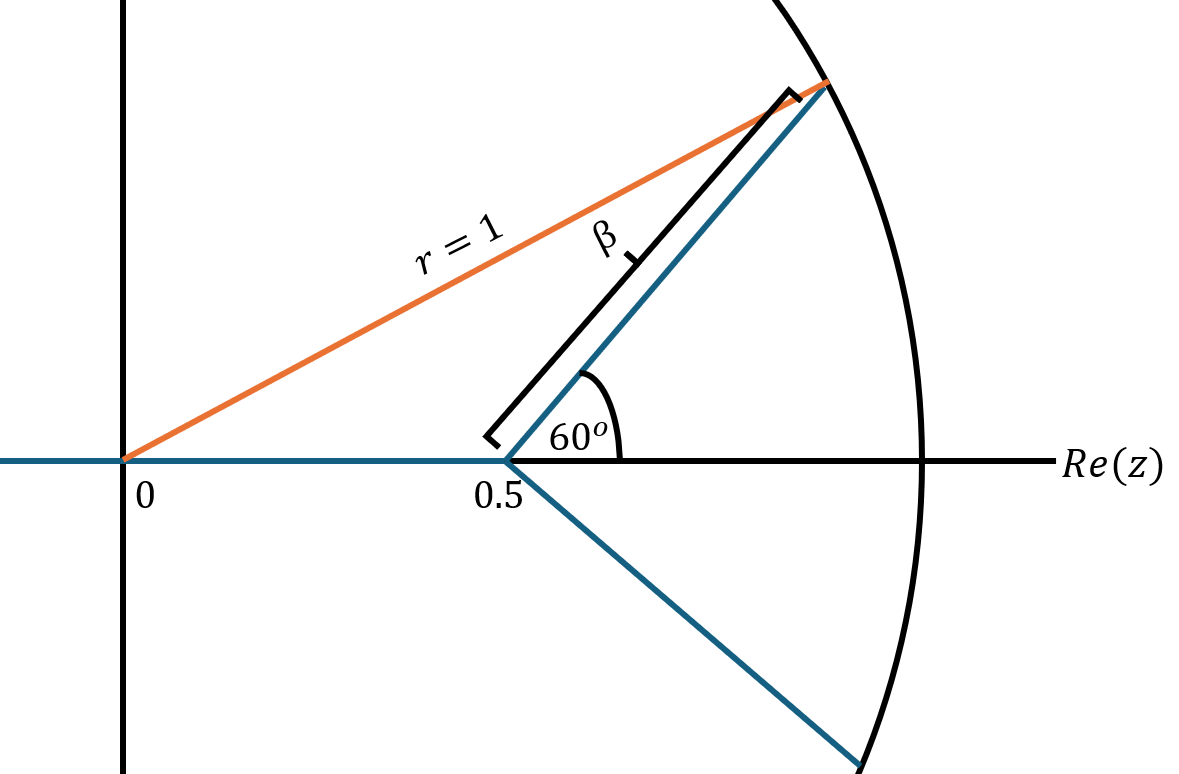
\includegraphics[width=0.5\textwidth]{Control_2_7.png}
    \captionof{figure}{LGR del sistema de lazo cerrado}
\end{center}
Aplicando por tanto trigonometria, se tendra que:
\begin{align}
    r\cdot cos(\theta)  = 0.5 + \rho cos(60^{\circ})\\
    rsen(\theta) = \rho sen(60^{\circ})\\
\end{align}
Sumando y elevando al cuadrado las expresiones anteriores se obtiene que:
\begin{align}
    1 = (0.5 + \rho cos(60^{\circ}))^{2} + \rho^{2}sen^{2}(60^{\circ})\\
    \rho = 0.6513
\end{align}
Con lo que el angulo asociado vendra dado por:
\begin{align}
    \theta = sen^{-1}(0.6513 \cdot sen(60^{\circ})) = 34.33^{\circ} = 0.5934[rad]
\end{align}
Con lo que se tendra que la frecuencia asociado asociada a esos polos corresponde a:
\begin{align}
    \omega_{n} = \frac{\theta}{T_{s}} = \frac{\theta}{10^{-3}} = 593.4[rad/s]
\end{align}
\subsection*{Resolucion (a-ii)}
Luego tenemos que si el polo es puramente real, se tendra necesariamente que $\theta_{1} = 0$ o $\theta_{2}= \pi$, recordando la formula del coeficiente tenemos que:
\begin{align}
    \xi = cos\left( tan^{-1} \left(\frac{\theta}{ln(r)}\right)\right)
\end{align}
Como sabemos de antemano que $\xi = 0.707$, se tendra que:
\begin{align}
    tan^{-1}\left(\frac{\theta}{ln(r)}\right) = \frac{\pi}{4}
\end{align}
Con lo que para cada caso de $\theta_{i}$ se tiene que:
\begin{align}
    \theta_{1} = 0 \rightarrow tan^{-1}(0)\in \left\{0, \pi , 2\pi \right\}\\
\end{align}
Por lo que se descarta este caso, para el caso de $\theta_{2}$ se tiene que:
\begin{align}
    \theta_{2} = \pi \rightarrow tan^{-1}\left(\frac{\pi}{ln(r)}\right)= \frac{\pi}{4} \rightarrow r = 0.0432
\end{align}
Con lo que finalmente se logra obtener el punto de diseño dado por:
\begin{align}
    z&= 0.0432 e^{j \pi} = -0.0432\\
    w_{n} &= \frac{1}{T_{s}} \sqrt{ln(r)^{2}+\theta^{2}} = 4443.111[rad/s]
\end{align}
Con lo que la ganancia necesaria vendra dada por:
\begin{align}
    K = \left| \frac{1}{\frac{1}{(z-0.5)^{3}}}\right|_{z=-0.0452} = 10.4911
\end{align}
\subsection*{Resolucion (b-i)}
Dado que se busca diseñar un controlador proporcional que entregue un coeficiente de amortiguamiento de $\xi = 0.56$, se puede aproximar el margen de fase a:
\begin{align}
    \xi = 0.56 \rightarrow MF = 56^{\circ}
\end{align}
Por lo tanto se tendra que:
\begin{align}
    MF_{deseado} = 180^{\circ} + \hat{MF} = 56^{\circ}\\
    \hat{MF} = -124^{\circ}
\end{align}
De esta manera se debe analizar las fases de la tabla entregada, tal que la suma de las fases de las plantas sea igual a -124, lo cual se cumple en aproximadamente 15 rad/s, donde se tiene que  $G_{1}(\omega_{c}) = 0.06537\angle(-78.69^{\circ} )$ y $G_{2}(\omega_{c}) = 0.04714\angle(-45^{\circ} )$. Finalmente dado que $|G(w_{c})|=1$ se concluye que:
\begin{align}
    k \cdot 0.06537 \cdot 0.04714 &= 1\\
    k &= 324.5129
\end{align}
\subsection*{Resolucion (b-ii)}
Dado que existe un retardo de una muestra, se tendra que el sistema vendra dado por:
\end{solution}
%-----------------------


\end{questions}
\newpage
%%%%%%%%%%%%%%%%%%%%%%%%%%%

\end{document}